%!TEX root=../book.tex

\chapter{\textit{t}-Tools}

\section{Overview of \textit{t}-Tools}

\subsection{One-Sample \textit{t}-Test}

The one-sample \textit{t}-test \index{$t$-test} \index{$t$-test!One sample} is one of the simplest entry points to inferential statistics there is. Simply put, it seeks to determine if the average value of a set of data differs significantly from some theoretical quantity. Say, for instance, we are working in a lumber mill and it looks like a shipment of Douglas fir trees is a bit smaller than usual. We know that a typical Douglas fir from this region is about 225 feet tall and has a radius of 7.5 feet, giving us a total volume of about $39000$ cubic feet.

So we take the measurements for each of the trees in this shipment and find that the average volume is $36500$ cubic feet with a standard deviation around $\sigma = 2000$ cubic feet. Do we have sufficient proof that these trees are actually smaller than our typical shipment?

Well, unfortunately, the human brain isn't great at intuitively figuring out if differences like that are meaningful or within the expected margin of error: that's where inferential statistics come into play. So let's first state our hypotheses as:
\begin{eqnarray*}
H_0:& \bar{x} = \mu\\
H_A:& \bar{x} \neq \mu
\end{eqnarray*}
where $\bar{x}$ is the mean volume of our shipment of trees and $\mu$ is the mean volume of adult Douglas firs. Now, we can conduct our statistical test.

A \textit{t}-test, speaking generally, takes the form:
\begin{equation}
t = \frac{\text{Estimate}-\text{Parameter}}{SE(\text{Estimate})}
\end{equation}
The specifics of what you plug in for the estimate and the parameter will vary a bit depending on which type of \textit{t}-test you use; however, they all are based off of this.

In our case, the one-sample \textit{t}-test will look like:
\begin{equation}
t=\frac{\bar{x}-\mu}{s_x}
\end{equation}
where each of the variables is what we defined in our hypotheses above. Plugging in our data we get:
\begin{eqnarray*}
t(124)&=&\frac{36500-39000}{2000/\sqrt{125}} \\
&=& -13.98
\end{eqnarray*}
Although we have our standardized \textit{t}-statistic, we still don't know if it reaches a level of significance or not. Historically, we would have to go to a table of \textit{p}-values and look up the one that was closest to our \textit{t}-statistic given the degrees of freedom (here, 124, or $n-1$). Thankfully, we now have software that is able to compute this value for us much more precisely and quickly. In this case, we end up with a \textit{p}-value $< 0.001$, showing that the result is highly significant.

\begin{figure}[htp]
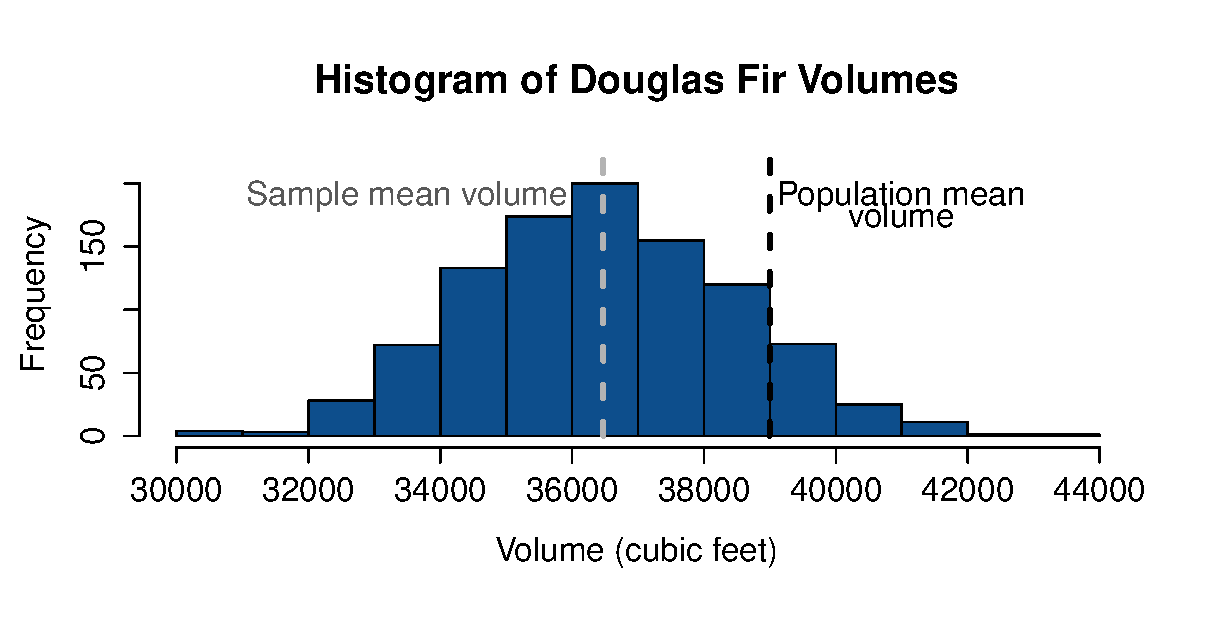
\includegraphics[width=\textwidth]{t01}
\caption{Histogram of the volumes of a shipment of Douglas firs with mean volume $36500$ cubic feet and standard deviation $\sigma = 2000$ cubic feet. A one-sample \textit{t}-test shows that this shipment of firs is significantly smaller than the typical shipment (mean $39000$ cubic feet), $t=-13.98$, $p\text{-value}<0.001$.}
\label{fig:t01}
\end{figure}

Moreover, we can infer the direction of this difference. Remember that the \textit{t}-statistic is computed by subtracting our estimated mean from our population mean: given this, a negative \textit{t}-statistic means that the sample mean is less than the population mean whereas a positive \textit{t}-statistic shows that our sample mean is greater than that of the population.

So, we can ultimately conclude that this shipment of Douglas firs is statistically significantly below the average size of a shipment, given $t(124)=-13.98$ with a $p\text{-value} < 0.001$. We can summarize this difference in Figure \ref{fig:t01}.

\subsection{Paired-Samples \textit{t}-Test}

So now that we're familiar with a one-sample \textit{t}-test \index{$t$-test!Paired samples}, the next two tests in the suite become really easy to understand. In a one-sample \textit{t}-test, we're testing one sample of data against a mean that we already know; with a paired-samples test, we extend that to two samples of data that are usually matched along some criteria. For instance, we might be looking at the difference in grieving patterns between mothers and fathers; or personality differences between heterozygous twins; or blood pressure of clinic patients before and after a given drug treatment.

In every case, our two variables are somehow \textit{related} to one another and for every data point in column A there is a corresponding data point in column B. For instance, let's say that we work at a large health clinic and we're testing a new drug, Procardia, that's meant to reduce hypertension. We find 1000 individuals with a high systolic blood pressure ($M=145$mmHg, $SD=9$), we give them Procardia for a month, and then measure their blood pressure again. We find that the mean systolic blood pressure has decreased to $138$mmHg with a standard deviation $8$. We can visualize this difference in Figure \ref{fig:t02}.

\begin{figure}[htp]
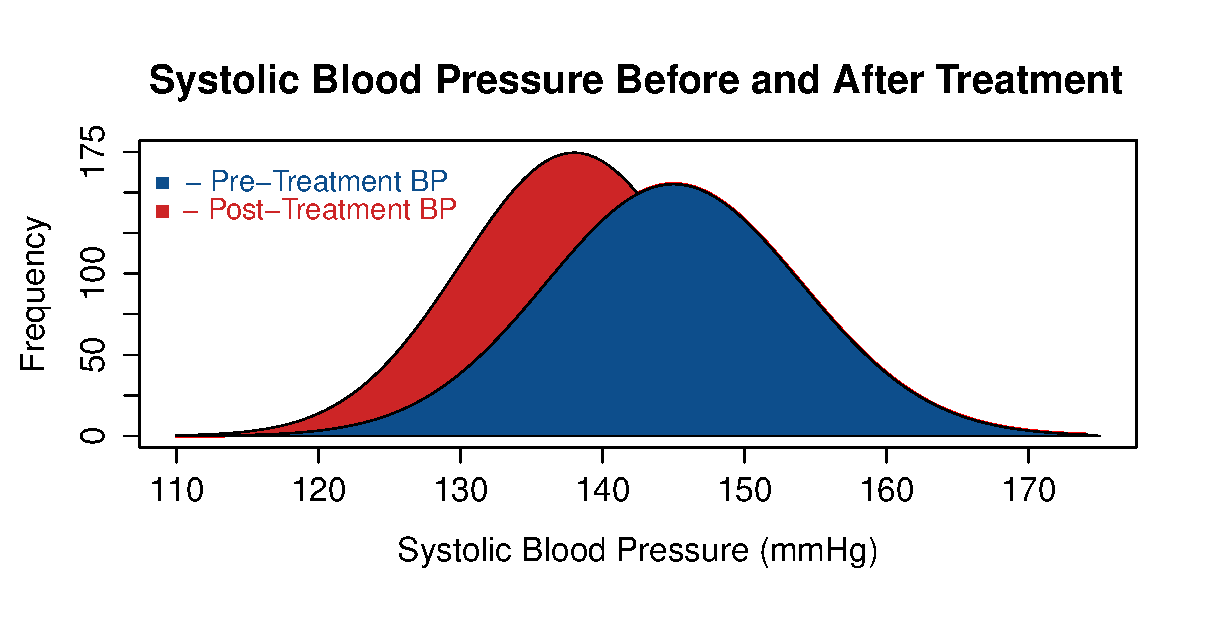
\includegraphics[width=\textwidth]{t02}
\caption{Systolic blood pressures before and after treatment with an antihypertensive drug.}
\label{fig:t02}
\end{figure}

So, we know that these data are paired: we used the same individuals for both pre-treatment and post-treatment and there are 1000 observations for each column of data. We know that the pre-treatment and post-treatment mean systolic blood pressures are different, but we want to know if this difference is statistically significant. In this case, our \textit{t}-test will take the form:
\begin{equation}
t=\frac{\bar{x}_1-\bar{x}_2}{s_{x_1-x_2}}\text{, where }s_{x_1-x_2}=\sqrt{\frac{s_1^2}{n_1}+\frac{s_2^2}{n_2}}
\end{equation}
Plugging in our data, we end up with $t(999)=19.75$, $p\text{-value}<0.001$, indicating that (yay!) our experimental drug does appear to actually reduce hypertension in individuals!

\subsection{Independent-Samples \textit{t}-Test}

Finally is the independent-samples \textit{t}-test \index{$t$-test!Independent samples}. Functionally, this is nearly identical to the paired-samples test: the only major difference is that it is used when the two samples are not paired or somehow related to one another. We would use this test if we were interested in determining, for example, whether there was a difference between depression scores of outpatients at two different clinics; or whether New Yorkers and Clevelanders spend different amounts of money each month eating out; or do two strains of a bacteria respond differently to an antimicrobial gel?

In each of these examples, there is no pairing: New Yorkers are an entirely different population from Clevelanders; the two strains of bacteria have been isolated from one another in a lab for generations. There aren't any obvious commonalities between the two samples.

Now, with this test, choosing the formula to use gets a little complicated. In fact, there are three that we can choose among. If both samples have an equal number of observations and equal variances, we use:
\begin{equation}
t = \frac{\bar {x}_1 - \bar{x}_2}{s_{x_1x_2} \cdot \sqrt{\frac{2}{n}}}\text{, where }s_{x_1x_2} = \sqrt{\frac{1}{2}(s_{x_1}^2+s_{x_2}^2)}
\label{eqn:t01}
\end{equation}
Alternately, if our samples have an unequal number of observations, but equal variances, we will use:
\begin{equation}
t = \frac{\bar {x}_1 - \bar{x}_2}{s_{x_1x_2} \cdot \sqrt{\frac{1}{n_1}+\frac{1}{n_2}}}\text{, where }s_{x_1x_2} = \sqrt{\frac{(n_1-1)s_{1}^2+(n_2-1)s_{2}^2}{n_1+n_2-2}}
\label{eqn:t02}
\end{equation}
Or, finally, we can use Welch's \textit{t}-test when the population variances are not assumed to be equal:
\begin{equation}
t = {\frac{\bar{x}_1 - \bar{x}_2}{s_{\bar{x}_1 - \bar{x}_2}}}\text{, where }s_{\bar{x}_1 - \bar{x}_2} = \sqrt{\frac{s_1^2}{n_1} + \frac{s_2^2}{n_2}}
\label{eqn:t03}
\end{equation}

Woah, that's a lot of choice. So, how do we figure out which to use, exactly? Well, it's not strictly speaking wrong to always default to using Welch's test \index{$t$-test!Welch's} assuming unequal variances. It's maybe not something that you necessarily \textit{should} always do, but it's better than using Equation \ref{eqn:t01} or \ref{eqn:t02} when the variances aren't actually equal. That said, we'll detail how exactly to determine which of these three tests to use in both the Equality of Variances and Implementation in R sections.

\section{Cautions and Considerations}

\subsection{Assumptions}

The suite of \textit{t}-tools assumes that:
\begin{enumerate}
\item the test variable is normally distributed;
\item the variances of the test variable are equal between the two populations;
\item the cases represent a simple random sample of the population; and
\item the scores on the test variable are independent of one another.
\end{enumerate}

\subsection{Equality of Variances}

As we mentioned above, the suite of \textit{t}-tools largely assumes that the variances \index{Equal variance} of the two samples are equal. However, when this is not actually the case, unless using Welch's test, your results can be a bit misleading. This difference arises from how each of the different tests computes the standard deviation for the two samples. Assuming unequal variances, the \textbf{pooled standard deviation} \index{Standard deviation!Pooled} is calculated.

By this estimate, the standard deviations of the two samples are combined (or pooled). However, these are first \textbf{weighted} by sample size. The idea behind this is that a standard deviation for a smaller sample doesn't carry as much importance as a standard deviation from a large sample. (The standard deviation of the large sample should be a better reflection of the population standard deviation.) Accordingly, each sample is weighted by its degrees of freedom.

Yet, if the two samples don't actually have the same standard deviation, this statistic quickly becomes misleading: it's like combining elephants and elephant mice together and calling them the same thing. Pretty obviously, they aren't. And once you start trying to make inferences about them, things are going to get wonky pretty quickly.

So before deciding which type of independent-samples test to run, we will first conduct Levene's test \index{Equal variance!Levene's test} for equality of variances. This operates under the hypotheses:
\begin{eqnarray*}
H_0:s_1=s_2 \\
H_A:s_1\neq s_2
\end{eqnarray*}
Without getting into the math behind it, the idea is that if it reaches a level of statistical significance, we can conclude that the two samples are not likely to actually have equal variances and we know to use Welch's test.

\subsection{Robustness of \textit{t}-Tools}

When we talk about the robustness of a test, we're talking about how well it holds up when we violate the assumptions that it relies on. Generally speaking, a more robust test is, of course, preferable: it allows us to still reach largely valid conclusions when some or all of our assumptions are not met.

When working with \textit{t}-tools, normality is generally not the biggest concern. As long as the sizes of your two samples are sufficiently large the test will remain valid, regardless of departures from normality. However, if both of the samples have the same standard deviation, these tests are moderately affected by long-tailedness (e.g., Figure \ref{fig:t04}).

\begin{figure}[htp]
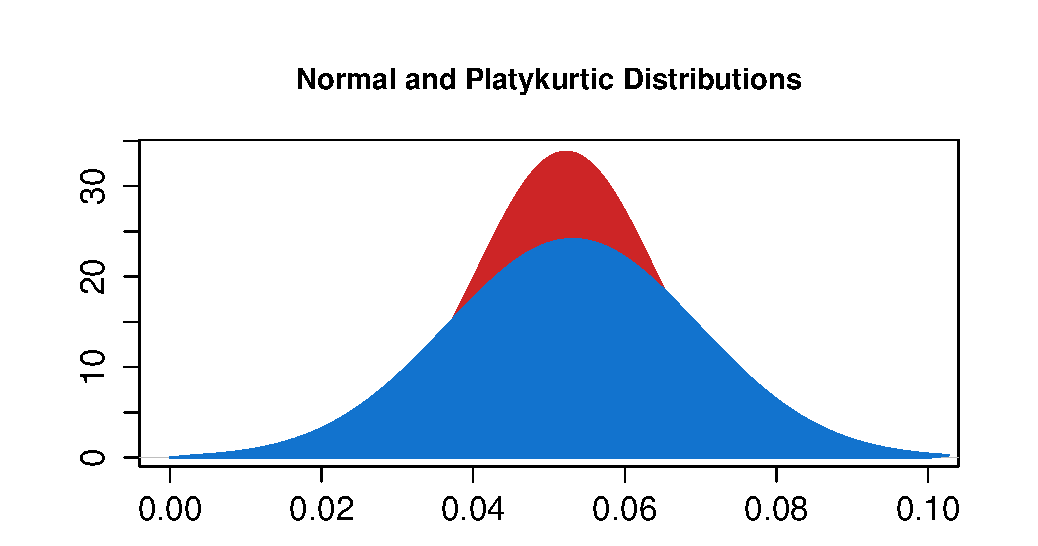
\includegraphics[width=\textwidth]{t03}
\caption{Two samples with the same standard deviation and approximately the same shape. One sample (blue) has longer tails. This moderately impacts the validity of \textit{t}-tools.}
\label{fig:t04}
\end{figure} 

If our assumption of independence, however, is violated, the \textit{t}-tool is likely to give misleading results. This assumption may be violated when there are cluster effects (samples come from the same cluster) or serial effects(samples are close together in time or space). 

\subsection{Resistance to Outliers}

We mentioned before (back when we introduced uncertainty, comparing the mean and median as measures of central tendency) the idea of resistance to outliers. The idea here is that a statistic or statistical procedure is resistant if the presence of one or a few outliers doesn't have an undue influence on the end result. In the case of means, outliers can significantly skew the result.

Unfortunately, because \textit{t}-tools are based on sample means, they are not resistant to outliers. If outliers are present in your data, it may be more appropriate to either remove them from the dataset or to use a comparable test that does not compare sample means. (These tests are usually called nonparametric tests: we detail some of them in the following chapter.)

\section{Implementation in R}
Please note: all data used in these explanations are simulated.

\subsection{One-Sample}
To conduct a one-sample \textit{t}-test in R, we use the syntax \verb|t.test(y, mu = 0)| where \verb|x| is the name of our variable of interest and \verb|mu| is set equal to the mean specified by the null hypothesis.

So, for example, if we wanted to test whether the volume of a shipment of lumber was less than usual ($\mu_0=39000$ cubic feet), we would run:
\begin{framed}
\begin{Verbatim}[samepage=TRUE]
# One-sample t-test
set.seed(0)
treeVolume <- c(rnorm(75, mean = 36500, sd = 2000))
t.test(treeVolume, mu = 39000) # Ho: mu = 39000
\end{Verbatim}
\end{framed}

\subsection{Paired-Samples}
To conduct a paired-samples test, we need either two vectors of data, $y_1$ and $y_2$, or we need one vector of data with a second that serves as a binary grouping variable. The test is then run using the syntax \verb|t.test(y1, y2, paired=TRUE)|

Going back to our example above using pre-treatment and post-treatment systolic blood pressures, our test would take the form:
\begin{framed}
\begin{Verbatim}[samepage=TRUE]
# Paired-samples t-test
# where y1 & y2 are numeric
set.seed(2820)
preTreat <- c(rnorm(1000, mean = 145, sd = 9))
postTreat <- c(rnorm(1000, mean = 138, sd = 8))
t.test(preTreat, postTreat, paired=TRUE)
\end{Verbatim}
\end{framed}

\subsection{Independent Samples}

The independent-samples test can take one of three forms, depending on the structure of your data and the equality of their variances. The general form of the test is \verb|t.test(y1, y2, paired=FALSE)|. By default, R assumes that the variances of \verb|y1| and \verb|y2| are unequal, thus defaulting to Welch's test. To toggle this, we use the flag \verb|var.equal=TRUE|.

In the three examples shown here we test the hypothesis that Clevelanders and New Yorkers spend different amounts monthly eating out. The first example assumes that we have two numeric vectors: one with Clevelanders' spending and one with New Yorkers' spending. The second example uses a binary grouping variable with a single column of spending data. (That is, there is only one column of spending data; however, for each dollar amount, the next column specifies whether it is for a New Yorker or a Clevelander.) Finally, the third example assumes that the variances of the two samples are unequal and uses Welch's test.
\begin{framed}
\begin{Verbatim}[samepage=TRUE]
# Independent-samples t-test
# where y1 and y2 are numeric
set.seed(0)
ClevelandSpending <- rnorm(50, mean = 250, sd = 75)
NYSpending <- rnorm(50, mean = 300, sd = 80)
t.test(ClevelandSpending, NYSpending, var.equal=TRUE)

# [...] where y1 is numeric and y2 is binary
spending <- c(ClevelandSpending, NYSpending)
city <- c(rep("Cleveland", 50), rep("New York", 50))
t.test(spending~city, var.equal=TRUE)

# with equal variances not assumed
t.test(ClevelandSpending, NYSpending, var.equal=FALSE)
\end{Verbatim}
\end{framed}

\section{Case Study: Medicare Spending on Patients}
The data used in this example were taken from \textit{Medicare hospital spending per patient} dataset, published by the Centers for Medicare and Medicaid Services, an agency of the Department of Health and Human Services.

Let's say that we're moving from New York to California and are interested in seeing how average Medicare spending per patient varies between the two states. We will first state our null and alternative hypotheses:
\begin{eqnarray*}
H_0&:&\mu_{\text{CA}}-\mu_{\text{NY}}=0 \\
H_A&:&\mu_{\text{CA}}- \mu_{\text{NY}}\neq 0 \\
\end{eqnarray*}
We're assuming that there is actually no difference in the mean Medicare spending per patient between the two states and are testing the hypothesis that a difference \textit{does} exist. We aren't specifying the direction of the difference (i.e., we aren't specifying which state we think will have a higher mean spending rate).

We can also visualize the spending patterns of the two states in Figure \ref{fig:t03}. Here, we see the Medicare spending per patient in each of the two states as a proportion of the national average spending per patient. (E.g., 1 represents the national average spending; 0.9 represents 90\% the national average spending, etc.)

\begin{figure}[htp]
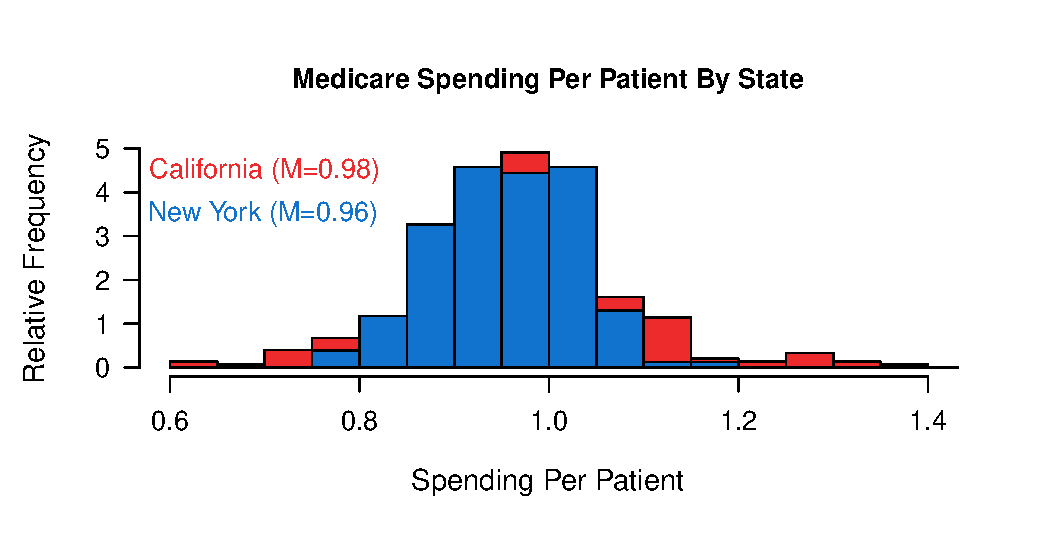
\includegraphics[width=\textwidth]{t04}
\caption{Medicare spending per patient in New York and California. Rates of spending are reported as a proportion of the national average Medicare spending per patient.}
\label{fig:t03}
\end{figure}

Next, we conduct Levene's test to see if we can assume equal variances or not:
\begin{framed}
\begin{Verbatim}[samepage=TRUE]
Levene's Test for Homogeneity of Variance (center = median)
       Df F value    Pr(>F)    
group   1  11.703 0.0006811 ***
      448  
\end{Verbatim}
\end{framed}

We see that there is significant evidence, $F=11.70$, $p\text{-value}<0.001$, that the variances of the two samples differ. Given this, we will go ahead and use Welch's test to evaluate our hypotheses. Doing so gives us the result:
\begin{framed}
\begin{Verbatim}[samepage=TRUE]
	Welch Two Sample t-test

t = 1.8277, df = 430.923, p-value = 0.06828
alternative hypothesis: true difference in means is not
                        equal to 0

95 percent confidence interval:
 -0.001252522  0.034494749

sample estimates:
mean in group CA  |  mean in group NY 
       0.9762290  |         0.9596078 
\end{Verbatim}
\end{framed}

So, here we have an interesting result: it looks like the two states \textit{might} have different mean spending levels per patient, $t=1.828$, $p\text{-value}=0.0683$; however, this doesn't quite reach our level of statistical significance. Moreover, if we look at the 95\% confidence interval provided, we see that the difference between the two population means is likely between -0.001 and 0.034, meaning that if there even is a difference between the two states, at most it's a difference of 3\% in per-patient spending relative to the national average.

Given this, we can conclude that although there may be a difference between the average per-patient Medicare spending of California and New York, that difference does not quite rise to the level of statistical significance. Further, even if there were a significant difference, there would not be a practical difference, as the two states are not likely to vary in spending by more than 3\% of one another.

\section{Exercises}

\section{Additional Resources}
